\documentclass[11pt,a4paper]{article}
\usepackage[margin=2.4cm]{geometry}
\usepackage{booktabs}
\usepackage{graphicx}
\usepackage{amsmath}
\usepackage{amssymb}
\usepackage[colorlinks=true,linkcolor=blue,urlcolor=blue]{hyperref}

\title{Cable hang: comparison of simulation methods\\
\large 3 supports, $L = 1.000$\,m,
$S = 0.800$\,m}
\author{Generated by \texttt{analysis/compare.py}}
\date{\today}

\begin{document}
\maketitle

\section{Setup}

A cable of length $L = 1.000$\,m hangs from
3 supports, all at the same height
$z = 1.000$\,m, evenly spaced across a horizontal span
$S = 0.800$\,m. Every method solves this identical scenario,
discretised into 60 segments, and each is initialised on
the analytic catenary so that what is measured is how far a solver
\emph{drifts} from equilibrium rather than how it recovers from an arbitrary
transient.

\paragraph{Cable.} $r = 2.00$\,mm,
$E = 80.0$\,MPa, $\nu = 0.45$,
$\rho = 2390$\,kg/m$^3$, mass $30.0$\,g
($\mu = 30.0$\,g/m), so
$EI = 1.005e-03$\,N\,m$^2$ and
$EA = 1.005e+03$\,N.

\section{Analytic reference}

For a perfectly flexible, inextensible cable on equal-height supports,
\begin{equation}
  z(x) = H + a\left[\cosh\!\left(\frac{x - S/2}{a}\right)
                    - \cosh\!\left(\frac{S}{2a}\right)\right],
  \qquad L = 2a\sinh\!\left(\frac{S}{2a}\right),
\end{equation}
with $a = T_0/w$ solved from the length constraint. Because all supports share
one height, the 3-support case separates exactly into
2 independent sub-catenaries of span
$S/2$ and length $L/2$.
For this scenario $a = 0.1691$\,m and the sag is
$132.7$\,mm.

\paragraph{Validity.} The catenary is the $EI \to 0$ limit. Bending competes
with gravity over the elasto-gravitational length
$\ell = (EI/w)^{1/3} = 150.5$\,mm. Here $\ell/S_{\mathrm{span}} = 0.376$, which is \emph{not} small. The catenary is being used outside its range of validity and the residuals below should be read as the physical difference between an elastic rod and an ideal chain, not as solver error.

\section{Results}

\begin{table}[htbp]
\centering
\small
\begin{tabular}{lrrrrrrc}
\toprule
Method & RMSE & max err & sag & sag err & arc drift & wall & settled \\
       & [mm] & [mm] & [mm] & [mm] & [\%] & [s] & \\
\midrule
    Newton cable (add\_rod + VBD) & 1.27 & 13.44 & 133.6 & 0.9 & 1.443 & 137.7 & -- \\
    PhysX capsule chain (D6) & 26.37 & 52.78 & 132.4 & -0.3 & -0.152 & 10.0 & -- \\
    Warp XPBD rod & 39.49 & 86.97 & 131.0 & -1.7 & -0.679 & 0.6 & \checkmark \\
\bottomrule
\end{tabular}
\caption{Every method against the analytic catenary. Reference sag
$132.7$\,mm. \emph{Arc drift} is the change in the cable's own
length during the run and is reference-free: it measures violation of
inextensibility directly.}
\end{table}

\begin{figure}[htbp]
  \centering
  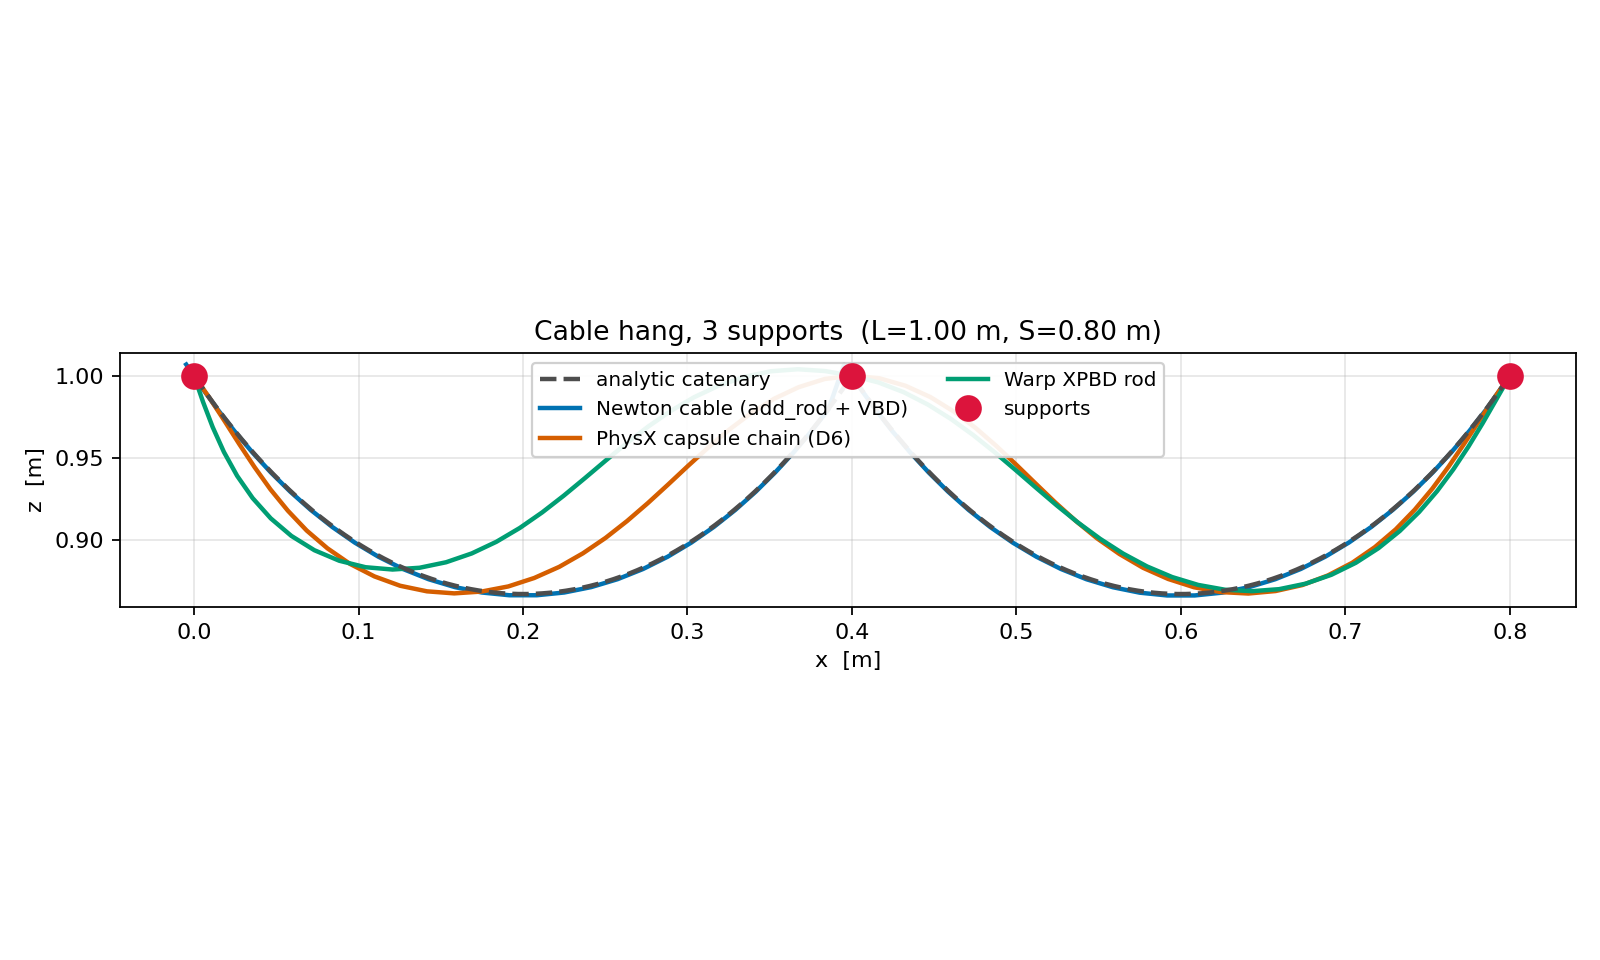
\includegraphics[width=\linewidth]{overlay.png}
  \caption{All methods against the analytic catenary.}
\end{figure}

\begin{figure}[htbp]
  \centering
  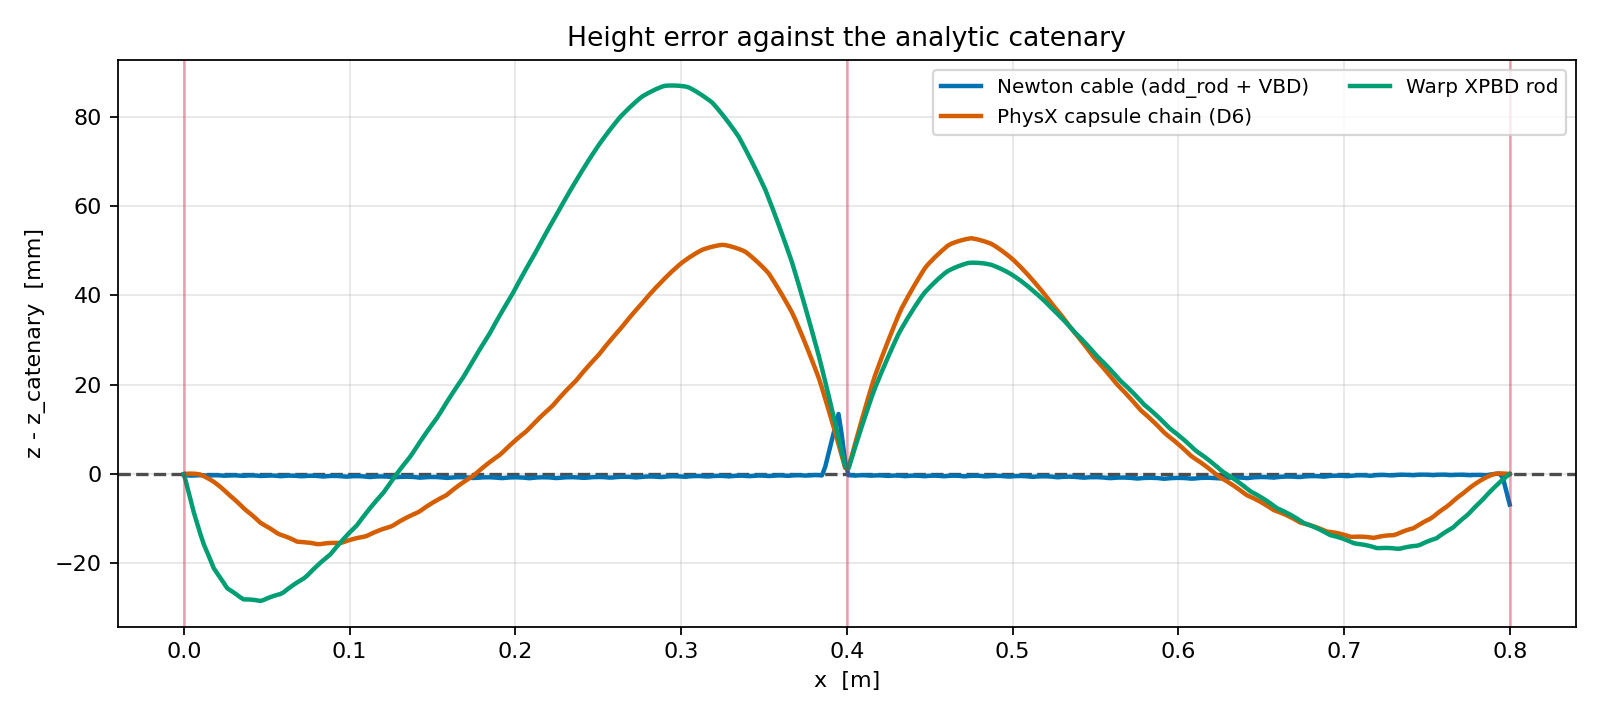
\includegraphics[width=\linewidth]{errors.png}
  \caption{Height error against the analytic catenary. Vertical lines mark the supports.}
\end{figure}


\section{Reading these numbers}

\begin{itemize}
  \item \textbf{Arc drift is the honest accuracy check.} It needs no
        reference shape. A solver that stretches the cable has failed
        regardless of how catenary-like its profile looks.
  \item \textbf{Agreeing with the catenary is not automatically a win.}
        Methods with no bending stiffness (a spherical-joint chain, for
        instance) match the ideal catenary because they share its idealisation,
        not because they model the cable more faithfully.
  \item \textbf{An unsettled run is provisional.} Where \emph{settled} is
        blank the motion had not decayed within the time cap, and the profile
        is a time-average over the final window rather than a true equilibrium.
\end{itemize}

\end{document}
